\documentclass{article}

%% If you want to number equations, set the equation number counter to zero.
%\setcounter{secnumdepth}{0}

\usepackage{amsmath,amssymb}
\usepackage[absolute]{textpos} %\usepackage[absolute,showboxes]{textpos}
\usepackage{graphicx}
\usepackage{natbib}
\usepackage{setspace}
%\usepackage{wrapfig}
\usepackage{times}
\usepackage[usenames]{color}
\definecolor{DarkBlue}{rgb}{0.1,0.1,0.5}
\definecolor{Black}{rgb}{0.0,0.0,0.0}
\definecolor{Red}{rgb}{0.9,0.0,0.1}
\definecolor{DarkBlue2}{rgb}{0.00,0.08,0.6}
\definecolor{DarkRed2}{rgb}{0.6,0.00,0.08}
\definecolor{DarkGreen2}{rgb}{0.00,0.6,0.08}
\usepackage{a0size}
\usepackage{floatflt}
\usepackage{pstricks}
\newrgbcolor{DarkBlue}{0.1 0.1 0.5}
\usepackage{pslatex}
\psset{linewidth=3pt}
\newcommand{\indep}{{\;\bot\!\!\!\!\!\!\bot\;}}

%%%%%%%%%%%%%%%%%%%%%%%%%%%%%%%% 
%%% NEW COMMAND DEFINTITIONS %%%
%%%%%%%%%%%%%%%%%%%%%%%%%%%%%%%%

%% See documentation for a0poster class for the size options here
%%    \normalsize will produce smaller type that might look too small
%%    \large will produce larger type
%% Feel free to modify if you want a different look
\let\Textsize\normalsize
%\let\Textsize\large
\def\RHead#1{\noindent\hbox to \hsize{\hfil{\huge\color{DarkBlue} #1}}\bigskip}
\def\LHead#1{\noindent{\veryHuge\color{DarkBlue} #1}\bigskip}
\def\CHead#1{\bigskip\begin{center}\noindent{\Large\color{DarkBlue} #1}\end{center}}
\def\Subhead#1{\bigskip \noindent{\large\color{DarkBlue} #1}}
\def\Title#1{\noindent{\textbf{\VeryHuge\color{DarkRed2} #1}}}

%%%%%%%%%%%%%%%%%%%%%%%%%%%%%
%%% GLOBAL LAYOUT OPTIONS %%%
%%%   NUMBER OF COLUMNS   %%%
%%%%%%%%%%%%%%%%%%%%%%%%%%%%%

%% Set paper size
%% Depending on the conference, the posterboard size may be different.
%% This template was based on an ISO standard A0, which is in use everywhere
%% except for the United States.  A0 paper is  46.81 in x 33.11 in.
%% Depending on the posterboard size and the printer, you may need to 
%% change the widths and margins here.  Text width and height are set
%% in terms of paper width and height -- you can change margins here.
\setlength{\paperwidth}{36in}
\setlength{\paperheight}{60in}
\setlength{\textwidth}{34in}    %% paperwidth - (3in)
\setlength{\textheight}{58in}   %% paperheight - (3in)
\special{papersize=\the\paperwidth,\the\paperheight}
\typeout{Paper width and height are \the\paperwidth and \the\paperheight}
\typeout{Text width and height are \the\textwidth and \the\textheight}
%% Margins
\setlength{\headheight}{0cm}
\setlength{\headsep}{0cm}
\setlength{\topmargin}{1in}
\setlength{\topskip}{0cm}
\setlength{\oddsidemargin}{1in}
\setlength{\evensidemargin}{0in}
%% Font sizes
\renewcommand{\tiny}{\fontsize{12}{14}\selectfont}
\renewcommand{\scriptsize}{\fontsize{14.4}{18}\selectfont}   
\renewcommand{\footnotesize}{\fontsize{17.28}{22}\selectfont}
%%\renewcommand{\small}{\fontsize{20.74}{25}\selectfont}
%%\renewcommand{\normalsize}{\fontsize{20.74}{25}\selectfont}
\renewcommand{\small}{\fontsize{24.88}{30}\selectfont}
\renewcommand{\normalsize}{\fontsize{29.16}{36}\selectfont}
\newcommand{\Normalsize}{\fontsize{36.08}{45}\selectfont}
\renewcommand{\large}{\fontsize{43}{54}\selectfont}
\renewcommand{\Large}{\fontsize{51.6}{64}\selectfont}
%\renewcommand{\LARGE}{\fontsize{43}{54}\selectfont}
\renewcommand{\huge}{\fontsize{61.92}{77}\selectfont}
%\renewcommand{\Huge}{\fontsize{61.92}{77}\selectfont}
\newcommand{\veryHuge}{\fontsize{68.85}{85}\selectfont}
\newcommand{\VeryHuge}{\fontsize{89.16}{134}\selectfont}
%\newcommand{\VERYHuge}{\fontsize{107}{134}\selectfont}
%% skip lengths
\setlength{\smallskipamount}{6pt plus 2pt minus 2pt}
\setlength{\medskipamount}{12pt plus 4pt minus 4pt}
\setlength{\bigskipamount}{24pt plus 8pt minus 8pt}
\setlength{\abovecaptionskip}{25pt}
\setlength{\belowcaptionskip}{0pt}
\setlength{\abovedisplayskip}{25pt plus 6pt minus 15 pt}
\setlength{\abovedisplayshortskip}{0pt plus 6pt}
\setlength{\belowdisplayshortskip}{13pt plus 7pt minus 6pt}
\setlength{\belowdisplayskip}{\abovedisplayskip}

\renewcommand{\refname}{}

%% Set up the grid
%%
%% Note that [40mm,40mm] is the margin round the edge of the page
%% it is _not_ the grid size. That is always defined as 
%% PAGE_WIDTH/HGRID and PAGE_HEIGHT/VGRID. In this case we use
%% 46 x 26. This gives us 4 columns of width 10 boxes, with a gap of
%% width 2 in between them.  There are 26 vertical boxes.
%%
%% (Note however that texblocks can be positioned fractionally as well,
%% so really any convenient grid size can be used.)
%%
\TPGrid[1in,1in]{38}{64}      % 4 cols of width 10, plus 3 gaps width 2

%% Text layout parameters
%%\parindent=0pt
\parskip=0.5\baselineskip

\hyphenation{mar-gin-als}


%%%%%%%%%%%%%%%%%%%%%%%%%%%%
%%% DOCUMENT BEGINS HERE %%%
%%%%%%%%%%%%%%%%%%%%%%%%%%%%

\begin{document}

%% Do not put page numbers at the bottom of the page for poster
\pagestyle{empty}

%% Border and background options -- you can make up others if you
%% like.  These all use the pstricks package.
%% DRAW A BLUE BORDER AROUND THE POSTER USING PSTRICKS
%%\psset{linewidth=0.5cm}
% Sets up lengths for frame
%%\newlength{\frameleft}
%%\newlength{\frameright}
%%\newlength{\frametop}
%%\newlength{\framebottom}
%%\setlength{\frameleft}{-1in}
%%\setlength{\frameright}{\textwidth}
%%\addtolength{\frameright}{1in}
%%\setlength{\frametop}{1in}
%%\setlength{\framebottom}{-\textheight}
%%\addtolength{\framebottom}{-1in}
% Draws a blue frame
%%\psframe[linecolor=darkblue,cornersize=absolute,linearc=2]
%%(\frameleft,\framebottom)(\frameright,\frametop)% need to overlay EOSMLS
%\psline{->}(0cm,0cm)(\textwidth,-\textheight)
%   *** End code to draw border *** 

%% USE A COLORED BACKGROUND FOR THE ENTIRE POSTER
%% [ADS 4-2005] THIS OPTION IS NOT SUPPORTED YET
%\newrgbcolor{gradbegin}{0.3 0.5 0.7}
%\newrgbcolor{LightBlue}{0.7 0.7 1.0}
%\psframe[fillstyle=solid,fillcolor=LightBlue](\frameleft,\framebottom)(\frameright,\frametop)



%% Adjust spacing in long displayed mathematical formulas to tighten them up
\setlength{\abovedisplayskip}{0.5\abovedisplayskip}
\setlength{\belowdisplayskip}{0.5\belowdisplayskip}


%% Understanding textblocks is the key to being able to do a poster in
%% LaTeX. The first argument gives the block width in grid cells, the
%% second gives the positioning on the grid.

\begin{textblock}{34}(1,00)
\Title{\vspace{0.4in}\texttt{eiPack}: Tools for R $\times$ C Ecological Inference\\
\mbox{$\quad\;\;\;$}and Higher-Dimension Data Management}
\end{textblock}

\begin{textblock}{6}(5,3.65)
\Subhead{Olivia Lau}
\end{textblock}
\begin{textblock}{6}(4.8,4.6)
{\Normalsize{\color{DarkBlue}olau@fas.harvard.edu}}
\end{textblock}

\begin{textblock}{6}(11.5,3.65)
\Subhead{Ryan T. Moore}
\end{textblock}
\begin{textblock}{6}(11.3,4.6)
{\Normalsize{\color{DarkBlue}rtmoore@fas.harvard.edu}}
\end{textblock}

\begin{textblock}{6}(19,3.65)
\Subhead{Michael Kellermann}
\end{textblock}
\begin{textblock}{6}(18.8,4.6)
{\Normalsize{\color{DarkBlue}kellerm@fas.harvard.edu}}
\end{textblock}

\begin{textblock}{30}(5.05,5.45)
\Subhead{\Normalsize{\textit{Department of Government and Institute for
Quantitative Social Science, Harvard University $\;$(Cambridge,
Massachusetts)}}}
\end{textblock}


%% Harvard logo on left, UseR Logo on right
\begin{textblock}{6}(30,-0.5)

\includegraphics[height=3.25in]{useR-large}
\end{textblock}
\begin{textblock}{6}(30,3.5)
\begin{flushright}
\Subhead{\color{DarkBlue}{Vienna, Austria}}
\end{flushright}
\end{textblock}
\begin{textblock}{6}(30,4.45)
\begin{flushright}
{\Normalsize\color{DarkBlue}{16 June 2006}}
\end{flushright}
\end{textblock}

\begin{textblock}{6}(-0.75,3.6)
\begin{center}

\includegraphics[width=2.5in]{Veritas_wreath_3C}
\end{center}
\end{textblock}

\begin{textblock}{38}(00,7.25)
\rule{34in}{4pt}
\end{textblock}



%% Begin first row
\begin{textblock}{12}(00,08)
\CHead{What is ecological inference ({\sc ei})?}
Goal:  infer individual level behavior from aggregate units
\begin{itemize}
\item Units of analysis are contingency tables with observed row and
column marginals.
\item {\sc ei} estimates unobserved internal cells for each unit.
\end{itemize} 
Let 
\begin{itemize}
\item $i = 1, \dots, n$ index units
\item $r = 1, \dots, R$ index the row marginals for each unit $i$
\item $c = 1, \dots, C$ index the column marginals for each unit $i$
\end{itemize}
For $R = 3$ and $C = 3$, each unit looks like ({\color{DarkRed2}{red
$=$ unobserved}}): 
\begin{center}
\begin{tabular}{l|ccc|c}
	& $col_1$ & $col_2$ & $col_3$ & \\
\hline
$row_1\quad$	& \color{DarkRed2}{$\quad N_{11i}\quad$} &
\color{DarkRed2}{$\quad N_{12i}\quad$} &
\color{DarkRed2}{$\quad N_{13i}\quad$} & $\quad N_{1\cdot i}$ \\
$row_2\quad$ 	& \color{DarkRed2}{$N_{21i}$} & \color{DarkRed2}{$N_{22i}$} &
\color{DarkRed2}{$N_{23i}$} & $\quad N_{2\cdot i}$ \\ 
$row_3\quad$	& \color{DarkRed2}{$N_{31i}$} & \color{DarkRed2}{$N_{32i}$} &
\color{DarkRed2}{$N_{33i}$} & $\quad N_{3\cdot i}$ \\ 
\hline
	& $N_{\cdot 1i}$ & $N_{\cdot 2i}$ & $N_{\cdot 3i}$ & $\quad N_i$
\end{tabular} 
\end{center}
The data may also be defined as fractions.  Let  
\begin{itemize}
\item Cell fractions be $\beta_{rci} = \frac{N_{rci}}{N_{r\cdot i}}$
\item Row marginals be $X_{ri} = \frac{N_{r\cdot i}}{N_i}$
\item Column marginals be $T_{ci} = \frac{N_{\cdot ci}}{N_i}$
\end{itemize} 

\CHead{Ecological regression}
\cite{goodman53} observes the identities 
\begin{eqnarray*}
T_{ci} = \sum_{r=1}^R \beta_{rci}X_{ri}  &\quad {\rm for } \quad& c =
1, \dots, C \quad {\rm and } \quad i = 1, \dots, n\\ 
\sum_{c=1}^{C} \beta_{rci}  =  1  &\quad {\rm for } \quad& r = 1, \dots, R
\quad {\rm and } \quad i = 1, \dots, n  
\end{eqnarray*}
Define the population cell fractions $\beta_{rc}$ such that
$\sum_{c=1}^{C} \beta_{rc}  =  1$ for every $r$.  Assuming that
$\beta_{rci} = \beta_{rc}$ for all $i$, estimating the regression equations
\begin{equation*}
T_{ci} = \beta_{rc} X_{ri} + \epsilon_{ci} \quad {\rm for } \quad c =
1, \dots, C\end{equation*}
recovers the population parameters $\beta_{rc}$ when the standard
linear regression assumptions apply, including $E[\epsilon_{ci}] = 0$
and $Var[\epsilon_{ci}] = \sigma_c^2$ for all $i$.
\end{textblock}

\begin{textblock}{12}(13,08)

\CHead{Method of bounds}
\cite{DunDav53} note that row and column marginals determine upper and lower
bounds on the possible proportion of row members in each column.
\begin{itemize}
\item In a unit, let $j$ be a given row and $K$ be the set of
all columns.  $K$ includes $k'$, the column of interest, $k''$, the
set of columns other than $k'$ included, and $\tilde{k}$, the set of columns excluded.
\item In the example below, consider the bounds on the proportion of
Native American two-party registrants who are Democrats: $j$ is Native American, $k'$ is
Democrat, $k''$ is Republican, and $\tilde{k}$ is No Party.
\item The quantity of interest can be written
\begin{displaymath}
\frac{N_{jk'}}{N_{jk'} + \sum_{k \in k''} N_{jk}}
\end{displaymath}
The lower and upper bounds on this proportion are given by
\begin{eqnarray*}
\textrm{Lower Bound: } & & \frac{\max(0, N_j - \sum_{k \neq k'}
N_k)}{\max(0, N_j - \sum_{k \neq k'} N_k) + \min(N_j, \sum_{k \in k''} N_k)} \\
\textrm{Upper Bound: } & & \frac{\min(N_j, N_{k'})}{\min(N_j, N_{k'}) + \max(0, N_j - N_{k'} - \sum_{k \in \tilde{k}} N_k)}
\end{eqnarray*}
\item Bounds tend to become more informative as homogeneity
increases within a unit;
\textit{extreme case analysis} centers on units satisfying row
thresholds such as ``60\% Native American precincts'' in the example below.
\end{itemize}
\end{textblock}


\begin{textblock}{12}(26,08)
\CHead{Multinomial-Dirichlet ({\sc md}) model}

\noindent \cite{RosJiaKin01} assume that the observed vectors of
column marginals are independent across units and the unobserved row vectors of
cell fractions are independent across rows and units.  
\begin{itemize}
\item Without covariate
\begin{eqnarray*}
(N_{\cdot 1i}, \dots, N_{\cdot Ci}) &\stackrel{\indep}{\sim}& {\rm Multinomial}(N_i,
\sum_{r=1}^R \beta_{r1i}X_{ri}, \dots, \sum_{r=1}^R \beta_{rCi}X_{ri}) \\
(\beta_{r1i}, \dots, \beta_{rCi}) &\stackrel{\indep}{\sim}& {\rm
Dirichlet}(\alpha_{r1}, \dots, \alpha_{rC})\\
\alpha_{rc} &\stackrel{\rm i.i.d.}{\sim}& {\rm
Gamma}(\lambda_1,\lambda_2) 
\end{eqnarray*}
\item With a covariate $Z_i$
\begin{eqnarray*}
(N_{\cdot 1i}, \dots, N_{\cdot Ci}) &\stackrel{\indep}{\sim}& {\rm Multinomial}(N_i,
\sum_{r=1}^R \beta_{r1i}X_{ri}, \dots, \sum_{r=1}^R \beta_{rCi}X_{ri}) \\
(\beta_{r1i}, \dots, \beta_{rCi}) &\stackrel{\indep}{\sim}& {\rm
Dirichlet}\left(d_r\exp(\gamma_{r1} + \delta_{r1}Z_i), \dots, \right. \\
& & \quad\quad \left. d_r\exp(\gamma_{r(C-1)} +
\delta_{r(C-1)}Z_i),\; d_r \right) \\
d_r &\stackrel{\rm i.i.d.}{\sim}& {\rm Gamma}(\lambda_1, \lambda_2)  
\end{eqnarray*}
\begin{itemize}
\item Priors on each $\gamma_{rc}$ and $\delta_{rc}$ are improper uniform
\item Parameterization of the prior on each $(\beta_{r1i}, \dots,
\beta_{rCi})$ is linear with respect to the covariate $Z_i$ in the
log-odds ratio of the expected fractions
\begin{displaymath}
\log\left( \frac{E(\beta_{rci})}{E(\beta_{rCi})} \right) = \gamma_{rc}
+ \delta_{rc} Z_i
\end{displaymath}
\end{itemize}
\end{itemize}
\end{textblock}

%% (x0,y0)(x1, y1) measured with origin in top left corner of poster
%% Exactly two columns wide.  x0 = -1.5, x1 = 21.6
\psframe[linecolor=DarkBlue,cornersize=absolute,linearc=1](10.4in,-20in)(33in,-26.75in)

\begin{textblock}{25.5}(13,23)
\CHead{Input-output for higher-dimension data objects}
\end{textblock}
\begin{textblock}{11.5}(13.5,24.5)
\begin{itemize}
\item Since units are tables, and the {\sc md} model allows for
inferences about the internal cells from the margins, each unit $i$
has $RC$ parameters, to yield a minimum of $RCn$ unit level parameters,
in addition to any population-level hyperparameters.  For $s$
simulations, the {\sc md} model yields a minimum of $RCns$ draws.  
\item In a state such as Ohio, for example, the {\sc
md} model requires (11,000 precinct $\times$ 3 party $\times$ 4 group)
parameter draws per simulation.  For 1,000 simulations, this is $1.32 \times
10^8$ unit-level draws, which occupy nearly 1GB of {\sc ram}, in
addition to population-level hyperparameters.  
\end{itemize}
\end{textblock}

\begin{textblock}{11.5}(26,24.5)
\begin{itemize}
\item Rather than storing unit-level parameters in the workspace, we
provide the option of saving each chain as a {\tt .tar.gz} file on
disk: 
\item[]{\small 
\begin{verbatim}
ei.MD.bayes(..., ret.beta = "s")
\end{verbatim}}
or discarding the unit-level draws entirely: 
\item[]{\small
\begin{verbatim}
ei.MD.bayes(..., ret.beta = "d")
\end{verbatim}}
\item To reconstruct the chains, users can select the row marginals,
column marginals, and units of interest:   
\item[]{\small 
\begin{verbatim}
read.betas(rows = c("black", "white"), 
   columns = c("dem"), units = 1:150, dir = getwd())
\end{verbatim}}
\end{itemize}
\end{textblock}


\begin{textblock}{38}(0,31.5)
\LHead{\texttt{eiPack} at work: Voter registration in southeastern North Carolina}
\end{textblock}


\begin{textblock}{12}(0,33)

\noindent{The models implemented in \texttt{eiPack} share}
\begin{itemize}
\item A common input syntax for each model of the form:
\begin{verbatim}cbind(col1, ..., colC) ~ cbind(row1, ...,rowR)\end{verbatim}
\item Functions to calculate shares for some subset of groups
\item Print and summary functions for each model
\end{itemize}
\noindent{To illustrate these methods, we use the \texttt{senc}
data  in \texttt{eiPack}:}
\begin{itemize}
\item Data on party affiliation of Black, White, and Native American
voters in eight counties (212 precincts) in SE North Carolina
\item Interior cell counts allow for model benchmarking
\end{itemize}

{\small
\begin{center}
\begin{tabular}{l|ccc|r}
      & Democrat & Republican & No Party & Total \\
\hline
Black & \emph{69999}        & \emph{3190}          &  \emph{5057}
& 78246 \\
White &  \emph{121941}  & \emph{97299}         &  \emph{41295}      & 260535 \\Native American & \emph{24480}     & \emph{1653}          &   \emph{1376}  & 27509 \\
\hline
Total  & 216420     & 102142        & 47728     & 366290
\end{tabular}
\end{center}}
\end{textblock}

\begin{textblock}{12}(0,42.2)
\CHead{Ecological regression}
\begin{itemize}
\item \texttt{ei.reg} performs the frequentist regression of column
marginals on row marginals:
\item[] {\small\begin{verbatim}
ei.reg(cbind(dem, rep, non) ~ cbind(black, white, natam), 
   data = senc)
\end{verbatim}}
\item \texttt{ei.reg.bayes} performs Bayesian regression of column
marginals on row marginals using the
improper prior $p(\beta, \sigma^2|X) \propto \sigma^{-2}$, which is uniform on $(\beta, \log \sigma)$:  
\item[] {\small\begin{verbatim}
ei.reg.bayes(cbind(dem, rep, non) ~ cbind(black, white, 
   natam), data = senc, sample = 1000, weights = NULL)
\end{verbatim}}
\item \texttt{lambda.reg} takes regression output and calculates
estimated proportions of row members falling in subsets of columns,
and standard errors around those estimates.  
\item[] {\small\begin{verbatim}
lambda.reg(out.reg, columns = c("dem", "rep"))
\end{verbatim}}
\item \texttt{density.plot} provides a graphical summary of \texttt{lambda} output:
\item[] {\small\begin{verbatim}
density.plot(lreg)
\end{verbatim}}
\item In the \texttt{senc} data, regression estimates of Black
and Native American two-party registration shares exceed the
possible limits.   
\end{itemize}
\end{textblock}

\begin{textblock}{6}(0,53.75)
\center \qquad Frequentist
\begin{center}
\includegraphics[width=5in]{ei.regress.eps}
\end{center}
\end{textblock}

\begin{textblock}{6}(6,53.75)
\center \qquad Bayesian
\begin{center}
\includegraphics[width=5in]{eiBayes.regress.eps}
\end{center}
\end{textblock}


\begin{textblock}{12}(13,32.5)

\CHead{Method of bounds}
\begin{itemize}
\item \texttt{bounds} calculates unit-level bounds on the proportion
of row members within a particular column: 
\item[] {\small\begin{verbatim}
bounds(cbind(dem, rep, non) ~ cbind(black, white, natam), 
   data = senc, rows = c("black", "natam"), column = "dem", 
   excluded = NULL, threshold = 0.6, total = NULL)
\end{verbatim}}
\item[] The \texttt{excluded} argument allows calculation of bounds on
proportions of a subset of columns.  Using \texttt{excluded = "non"}
above would calculate the bounds on the share of two-party
registration.
\item \texttt{plot} graphically displays the bounds for one row and
highlights the intersection (if any) of the plotted bounds:
\item[] {\small\begin{verbatim}
plot(out, row = "natam", column = "dem", intersection = T)
\end{verbatim}}
\item In the \texttt{senc} data, the lower bound for Democratic
registration among Native Americans is greater that 0.8 in most of the
60\% Native American precincts.  Values between 0.93 and 0.96 are
possible in all of these precincts.
\end{itemize}
\begin{center}
\includegraphics[height=10in]{bounds.eps}
\end{center}
\end{textblock}

\begin{textblock}{12}(13,53.5)
\begin{center}
\rule{8in}{2pt}
\end{center}
\begin{center}\Subhead{Acknowledgments}\end{center}
{\small Thanks to Gary King, Kevin Quinn, and D. James Greiner for
suggestions, Matt Cox and Bob Kinney for technical advice, and the
Institute for Quantitative Social Science for travel funding. }
\begin{center}\Subhead{References}\end{center}
\end{textblock}




\begin{textblock}{12}(26,30)
\begin{center}
%%%%\caption{Counties included in \texttt{senc}}
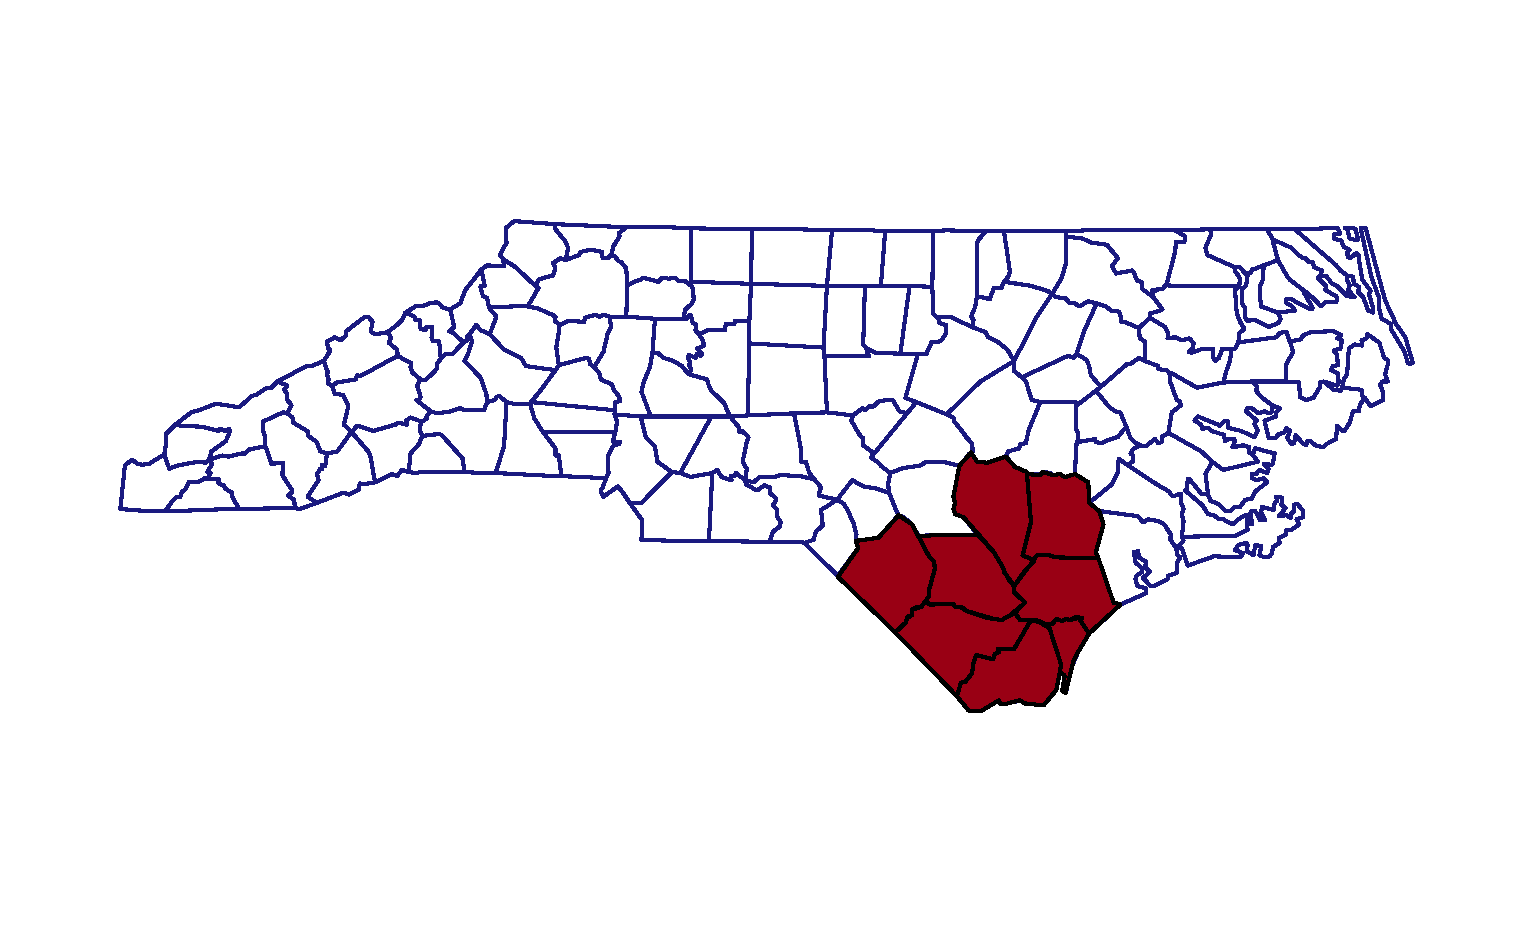
\includegraphics[width=10in]{ncmap.eps}
\end{center}
\end{textblock}
\begin{textblock}{12}(26,36.5)
\CHead{Multinomial-Dirichlet ({\sc md}) model}

\begin{itemize}
\item \texttt{tuneMD} calibrates the tuning
parameters used for Metropolis-Hastings sampling:
\item[] {\small\begin{verbatim}
tuneMD(cbind(dem, rep, non) ~ cbind(black, white, natam), 
   data = senc, ntunes = 10, sample = 1000, 
   thin = 1000)
\end{verbatim}}
\item \texttt{ei.MD.bayes} is the primary model-fitting function,
calling \texttt{C} code to generate MCMC draws.  Users
can
\begin{itemize}
\item return precinct parameters, discard, or save to disk
\item return parameters as \texttt{mcmc} objects or arrays
\item define a function to operate on each iteration within \texttt{C}
\end{itemize}
\item[] {\small
\begin{verbatim}
ei.MD.bayes(cbind(dem, rep, non) ~ cbind(black, white, 
   natam), covariate = NULL, data = senc, lambda1 = 4, 
   lambda2 = 2,  tune.list = tune.nocov, start.list = NULL, 
   sample = 1000, thin = 5000, burnin = 1000000, 
   ret.beta = 'r', ret.mcmc = TRUE, usrfun = NULL)
\end{verbatim}}
\item Usage for \texttt{lambda.MD} and \texttt{density.plot} is analogous to
ecological regression:
\item[] {\small\begin{verbatim}
lambda.MD(out.nocov, columns = c("dem", "rep"))
density.plot(lmd)
\end{verbatim}}
\item If precinct parameters are returned or saved, \texttt{cover.plot}
plots the central credible intervals for each precinct:  
\item[]{\small\begin{verbatim}
cover.plot(out.nocov, row = "white", column = "dem")
\end{verbatim}}
\item In the \texttt{senc} data, comparing the estimated precinct
parameters to the true values shows that the percentage of White Democrats is
underestimated in precincts with few White voters.
\end{itemize}
\end{textblock}

\begin{textblock}{12}(26,51.5)
\begin{center}
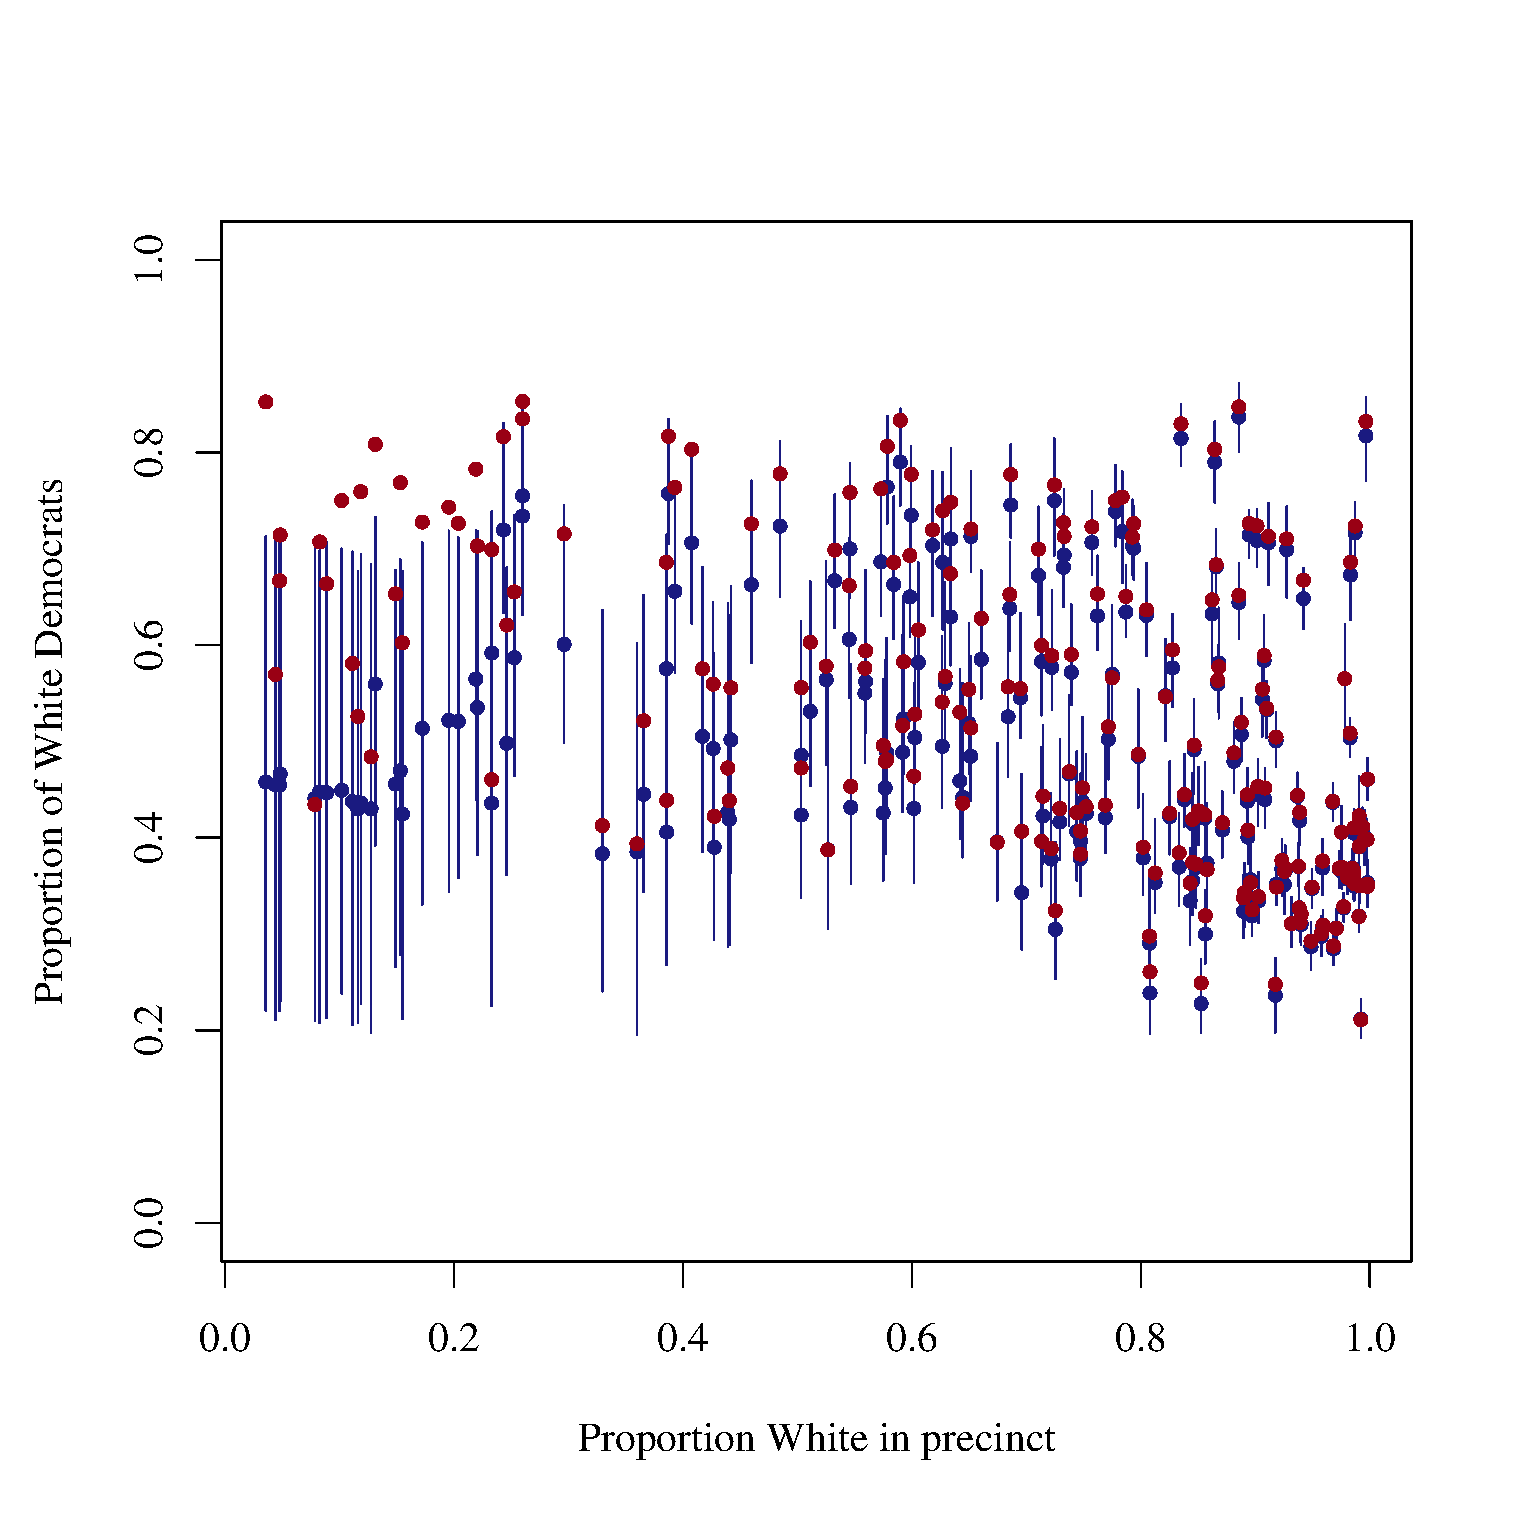
\includegraphics[width=10in]{cover.nocov.eps}
\end{center}
\end{textblock}


\begin{textblock}{12}(13,57.5)
{\small
\bibliographystyle{apsr}
\bibliography{ei}
}
\end{textblock}


\begin{textblock}{38}(00,63)
\rule{34in}{4pt}
\end{textblock}


%%\begin{textblock}{10}(36,15)
%%\CHead{Making a poster backup}
%%The \texttt{textblock} environments here transfer easily to slide
%%presenation packages for \LaTeX, such as \texttt{prosper}, \texttt{beamer},
%%and \texttt{slitex}.  Since the layout of the poster in this document is
%%a logical one, you can simply mimic that in your favorite slidemaking
%%package to obtain letter-sized sheets to use as a backup in case this
%%poster is is missing, damaged, incorrectly-sized, etc.
%%\\
%%\\
%%\CHead{New Heading}
%%Let's see if this works right.
%%
%%\end{textblock}


%%\begin{textblock}{10}(36,21)
%%\bibliographystyle{plain}
%%\bibliography{posterTemplate}
%%\end{textblock}



\begin{textblock}{38}(00,58)
\begin{center}
{\footnotesize 
\vspace{-0.75\baselineskip}
}
%%{\footnotesize Acknowledgments: This work was performed while the
%%author held a National Defence Science and Engineering Graduate
%%Fellowship.  This template was modified only slightly from that of Ron
%%Kumon in order to make it more specifically a tutorial for the
%%Berkeley Wireless Foundations Center.}
\end{center}
\end{textblock}



\end{document}
